\documentclass[11pt, wide]{article}
    \usepackage[utf8]{inputenc}
    \usepackage[T1]{fontenc}    
    \usepackage{polski}
    
    \usepackage{graphicx}
    \usepackage{caption}
    \usepackage{subcaption}
    \usepackage{epstopdf}
    
    \usepackage{hyperref}
    \usepackage{url}
    \usepackage{bbm}
    \usepackage{comment}
    \usepackage{makecell}
    \usepackage{xcolor}
    \usepackage{listings}
    \usepackage{secdot}

    \definecolor{mGreen}{rgb}{0,0.6,0}
    \definecolor{mGray}{rgb}{0.5,0.5,0.5}
    \definecolor{mPurple}{rgb}{0.58,0,0.82}
    \definecolor{backgroundColor}{rgb}{0.95,0.95,0.92}
    \lstdefinestyle{CStyle}{
        backgroundcolor=\color{backgroundColor},
        commentstyle=\color{mGreen},
        keywordstyle=\color{magenta},
        numberstyle=\tiny\color{mGray},
        stringstyle=\color{mPurple},
        basicstyle=\footnotesize,
        breakatwhitespace=false,
        breaklines=true,
        captionpos=b,
        keepspaces=true,
        numbers=left,
        numbersep=5pt,
        showspaces=false,
        showstringspaces=false,
        showtabs=false,
        tabsize=2,
        language=C
    }

    \author{Łukasz Klasiński}
    \date{Wrocław, \today}
    \title{\LARGE\textbf{Dokumentacja projektu z \\Baz Danych\\}
    Prowadzący : Jan Otop}
    \begin{document}
    \maketitle
    \thispagestyle{empty}
    \section{Diagram E-R - model konceptualny}
    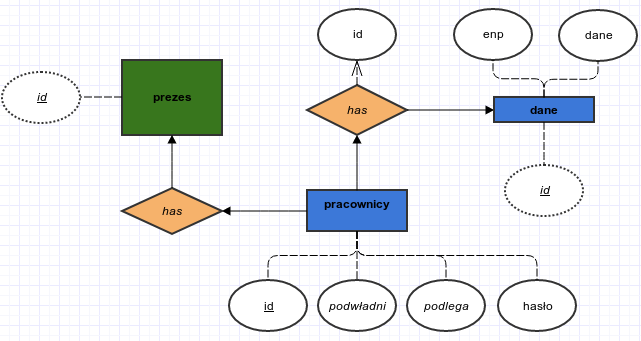
\includegraphics[width=\textwidth]{er}    

    Diagram pokazuje koncept bazy dla danego problemu. Atrybut \textit{podwładni}
    ze zbioru \textbf{pracownicy}, oznaczaja wszystkich bezpośrednio podległych pracowników. Z kolei
    \textit{podlega} pracowników, którym bezpośrednio lub pośrednio podlega. 
    Encja \textbf{prezes} zawiera pojedyńczy wpis, zawierający \textit{id} pracownika, który
    jest prezesem.\\

    Użytkownik \textbf{\textit{app}} ma możliwość odczytu oraz zapisu encji pokolorowanych
    na niebiesko, tylko odczytu dla zielonych tabel. Z kolei \textbf{\textit{init}} ma dostęp do całej bazy danych.

    \section{Implemetacja}
    Funkcje dodające/modyfikujące użytkowników będą wykonywać standardowe
    funkcje \textit{SELECT} oraz \textit{UPDATE} języka sql, ze sprawdzaniem, czy 
    dany użytkownik posiada odpowiednie prawa.\\\\       
    Funkcje szukające pracowników, którym dana osoba podlega będą zwracać wartości zawarte w liście \textit{podlega}.\\\\ 
    Znajdowanie wszystkich podległych pracowników, szuka w bazie danych wpisów z podaną wartością \textit{emp} w liście \textit{podlega} 
    znajdującą się na miejscu równym głębokości wystąpienia szukanej osoby w drzewie. \\\\
    Usuwanie pracownika, rekurencyjnie usuwa dane kolejnych pracowników.\\\\
    Tworzenie wpisu prezesa dodatkowo dodaje odpowiedni wpis do tabeli \textit{prezes}.

    \section{Wymagania}
    Api wymaga zainstalowanego interpretera języka \textbf{Python} w wersji co najmniej
    \textbf{2.7} oraz zainstalowanego modułu \textbf{psycopg2} w wersji przynajmniej \textbf{2.7.2}.
    Poza tym api korzysta z silnika baz danych \textbf{Postgresql} w wersji $\geq$ \textbf{9.1.23}
    z zainstalowanym modułem \textbf{pgcrypto}. 

    \section{Uruchomienie}
    Spośród zawartych plików należy uruchomić za pomocą interpretera python plik \textbf{api.py}, który 
    po uruchomieniu będzie czekać na standardowym wejściu na zgodne ze specyfikacją danych 
    do napotkania znaku końca lini. Dla każdego zapytania program zwraca dwie możliwe wartości w formacie JSON:

    \begin{itemize}
    \item  \begin{lstlisting}[style=CStyle] 
        {"status" : "OK" , "data" : [ "v1", "v2",...]}\end{lstlisting}
        W przypadku powodzenia,  gdzie zawartość pole \textit{data} jest opcjonalne i występuje tylko przy zapytaniach
        oczekujących na wynik. Poszczególne dane wynikowe są zawsze w tablicy. Oznacza to, że dla wyników
        jednoelementowych zwrócona zostanie tablica jednoelementowa. Ponadto kolejne wartości 
        \textit{$v_i$} są zawsze ciągami tekstowymi, nawet w przypadku wartości boolowskich, np: 
        \textit{"data" : ["false"]} może być wynikiem dla zapytania \textit{ancestor}. Jest to 
        zastosowane w celu unifikacji danych wyjściowych. Ponieważ wszystkie wartości na wejściu 
        są traktowane oraz zapisywane jako stringi, zwracane dane także nimi są. W szczególności dzięki temu
        unikatowe identyfikatory pracowników \textit{emp} mogą być dowolnymi typami danych.
    \item \begin{lstlisting}[style=CStyle]
        {"status" : "ERROR", "debug" : "opis"}\end{lstlisting}
        W przypadku błędu, gdzie \textit{debug} zawiera opcjonalne informacje o przyczynie błędu.
        Przykładowo \textit{Wrong admin password} oznacza, że podane zostało nieprawidłowe hasło 
        dostępu do aplikacji.  Dodatkowo jeśli błąd nie był spowodowany błędnymi danymi, tylko błędem bazy danych,
        to jego wynik zostanie umieszczony w polu \textit{debug}. W szczególności, jeśli  przypadkowo dwa razy
        poda zapytanie z parametrem \textit{init}, to zwrócony zostanie błąd silnika bazy danych informujacy o tym, że 
        tablice, które próbuje utworzyć api już istnieją. 
    \end{itemize}


    Przykładowe uruchomienie:
    \begin{lstlisting}[style=CStyle]
    python api.py\end{lstlisting}    
    Dodatkowo w systemach uniksowych, można po nadanu odpowiednich praw uruchomić plik \textit{api.py} 
    jako plik wykonywalny:
    \begin{lstlisting}[style=CStyle]
    chmod +x api.py
    /.api.py\end{lstlisting}


\end{document}

